\documentclass[12pt]{article}
\usepackage[T1]{fontenc}
\usepackage{calc}
\usepackage{setspace}
\usepackage{multicol}
\usepackage{fancyheadings}

\usepackage{graphicx}
\usepackage{color}
\usepackage{rotating}
%\usepackage{harvard}
%\usepackage{aer}
%\usepackage{aertt}
\usepackage{verbatim}
\usepackage{natbib}

\setlength{\voffset}{0in}
\setlength{\topmargin}{0pt}
\setlength{\hoffset}{0pt}
\setlength{\oddsidemargin}{0pt}
\setlength{\headheight}{0pt}
\setlength{\headsep}{0in}
\setlength{\marginparsep}{0pt}
\setlength{\marginparwidth}{0pt}
\setlength{\marginparpush}{0pt}
\setlength{\footskip}{.2in}
\setlength{\textwidth}{6.5in}
\setlength{\textheight}{9in}
\setlength{\parskip}{0pc}

\renewcommand{\baselinestretch}{1.0}

\newcommand{\bi}{\begin{itemize}}
\newcommand{\ei}{\end{itemize}}
\newcommand{\be}{\begin{enumerate}}
\newcommand{\ee}{\end{enumerate}}
\newcommand{\bd}{\begin{description}}
\newcommand{\ed}{\end{description}}
\newcommand{\prbf}[1]{\textbf{#1}}
\newcommand{\prit}[1]{\textit{#1}}
\newcommand{\beq}{\begin{equation}}
\newcommand{\eeq}{\end{equation}}
\newcommand{\beqa}{\begin{eqnarray}}
\newcommand{\eeqa}{\end{eqnarray}}
\newcommand{\bdm}{\begin{displaymath}}
\newcommand{\edm}{\end{displaymath}}
\newcommand{\script}[1]{\begin{cal}#1\end{cal}}
\newcommand{\citee}[1]{\citename{#1} (\citeyear{#1})}
\newcommand{\h}[1]{\hat{#1}}
\newcommand{\ds}{\displaystyle}

\newcommand{\app}
{
\appendix
}

\newcommand{\appsection}[1]
{
\let\oldthesection\thesection
\renewcommand{\thesection}{Appendix \oldthesection}
\section{#1}\let\thesection\oldthesection
\renewcommand{\theequation}{\thesection\arabic{equation}}
\setcounter{equation}{0}
}

%\pagestyle{fancyplain}
%\lhead{}
%\chead{Students' Thought Processes For Choosing Appropriate Statistical Methods}
%\rhead{\thepage}
%\lfoot{}
%\cfoot{}
%\rfoot{}

\pagestyle{fancyplain}
\lhead{}
\chead{}
\rhead{}
\lfoot{}
\cfoot{}
\rfoot{\thepage}
\renewcommand{\headrulewidth}{0pt}

\usepackage[none]{hyphenat}
%\hyphenpenalty=100000


\begin{document}

\section{Introduction}

In introductory statistics classes, students are typically drilled on the procedures to implement a variety of statistical tests.  Even when successful in this class, it is possible to struggle in subsequent research methods classes when asked to select an appropriate statistical test to investigate a research question.  This requires an advanced organization of knowledge of statistical tests which reflects an understanding of how statistical methods are related to one another.  

Experts organize this knowledge along several dimensions: univariate versus multivariate techniques; parametric versus non-parametric tests; tests appropriate for variables with different scales of measurement (nominal, ordinal, interval/ratio); and tests with different goals, for example investigating differences, relationships, independence, etc.  When experts are given some basic information about a research question and the available data, they take advantage of one or more of these mental mappings and draw from memory an appropriate statistical procedure for the research question.  More often, experts are presented only with a research question, and then tackle the more complicated problem of simultaneously choosing what variables are relevant and how they should be measured, and what statistical procedure to use.  

For the expert, these complicated cognitive processes have been developed and practiced with years of experience, and these choices can therefore be made easily.  A student who is a novice in statistics needs to be carefully guided along this decision making process.  \citet{ambrosebook} suggests that when students begin developing knowledge organizations, the connections are often superficial, or otherwise structured in a way that is not effective for applying a body of existing knowledge to new situations.  In a number of papers, \citeauthor{ausubel1978} finds statistical evidence that learning is improved when students are presented with a way to organize knowledge as they learn new concepts.\footnote{See \citet*{ausubel1978} for a review and defense of his many contributions on organizing knowledge and student learning.}  It is our responsibility as instructors to recognize the cognitive hurdles students face when asked to apply statistics to research questions, and to help students develop a knowledge organization that facilitates this task.  

The purpose of this paper is to share our classroom experience in helping students develop a way to organize knowledge of statistical techniques.  In doing so, we describe our classroom presentation for how to organize knowledge of statistical tests.  We expose our students' thought processes for selecting statistical tests, before, during, and after this intervention and describe common points of confusion our students encountered.  Finally, we report on our students' performance in selecting appropriate statistical tests both before and after our treatment, and suggest teaching improvement strategies.

In the literature on the teaching and learning of statistics, there is relatively little on organizing knowledge or on training students how to choose statistical tests.  This issue has been recently addressed in the medical education literature.  \citet{medpaper} focus on some common statistical techniques in medical studies and present some decision trees to guide students on how to choose an appropriate statistical test.  These decision trees are confined to two criteria: the scale of measurement for the test variable (continuous, binary, or categorical), and whether the research design is paired or not paired.  The present paper expands on this idea.

While little else in the literature addresses the specific idea of organizing knowledge of statistical tests, a larger number of papers speak more generally to the importance of investigating this critical thinking process.  \citet*{garfield2000} note that there is a growing movement in statistics courses' learning outcomes to also focus on critical thinking skills.  \citet*{pantang} find that an application approach to teaching leads to less student anxiety.  For example, a focus on actual research papers and examples in daily life allowed students to dispel the myths that there are not meaningful uses of the course content and that statistics is only useful for those with superior math skills.  \citet*{mvududu2005} makes the case that instructors should help students take what they already know and use it to create new knowledge.  He furthermore suggests that instructors should study how students think about the material they encounter and investigate students' thought processes on a deeper level than through everyday communication.  This is precisely the contribution we make in this paper.

We accomplish this goal by reporting on a lesson study that we conducted in our classrooms during the 2011-2012 academic year.  A lesson study is a teaching improvement activity in which instructors jointly develop a lesson to make the students' learning processes visible, then observe the students and record their observations.  Lesson study is a standard practice in Japanese elementary education, and it has recently been introduced to higher education in the United States by \citet*{cerbinkopp} and elaborated on in \citet*{cerbinbook}.  By focusing on a single lesson, instructors can look deeply into every step of the teaching and learning process: from the goals of a given teaching activity, to the design of the classroom instruction, to understanding the students' reception and mental processing of the class content, and finally to making evidence-based improvements.  In the forward to \citet*{cerbinbook}, Pat Hutchings uses the following words to describe his lesson study experience in an introductory level psychology course, ``We were immersed in something very different from other teaching improvement activities... each week we questioned our basic assumptions about teaching and thought about the essential goals of the psychology course, what students should really understand, and the learning problems students experience.''  In this paper we share a similar experience from our research methods course.  While we expected some sources of confusion for our students, we were surprised by others, including the difficulty students had identifying what constituted a variable, difficulty with statistical and colloquial language, and difficulty understanding the difference between paired-samples and independent samples.  We reflect on these problems and suggest how to address these common points of confusion. 

The goals for lesson study are somewhat different than other scholarly work in teaching and learning.  The intention is to make evidence-based improvements in the lesson design.  Still, even a lesson that is identified in hindsight as imperfect can offer valuable insight into how students process new information, and it can provide direction on more effective teaching strategies to pursue in the future.   Sharing a lesson study design and its findings can also facilitate lesson study development for other instructors, especially for lessons with related content.  In our lesson study project, we expose students' pre-existing thought processes for choosing a statistical test, we witness how this thought process evolved after giving students a way to organize this knowledge, and we suggest how to address common difficulties that our students encountered. 

\section{Lesson Design}

Each of the two authors of this paper taught separate sections of a business research methods course in Fall 2011 and Spring 2012.  Throughout the statistics portion of the course, we taught our students how to identify a statistical test to answer a research question.  We emphasized the consideration of the research question to be answered, the number of variables, the scale of measurement of the variables, whether observations were independent or paired, and whether the goal of the research question was to test for differences between groups or relationships/comovement between variables.  We had regular discussions on our teaching approaches for this part of the class and we each used multiple examples in each of our courses.  Still, we did not make an explicit attempt to make the actual presentation of the material identical, so our students' performance may have still been influenced by instructor-specific effects.

For our classroom observation, we jointly developed a single class period lesson on how to organize statistical knowledge, which included a brief lecture and four in-class exercises (all of which are included in Appendix A).  Each exercise presented a student with a description of a single research question and survey data which could be used to answer it.  The exercise asks the students to choose an appropriate statistical test to answer the research question, describe aspects of the the scenario that led them to this decision, and finally report how confident they are in their answer on a three-point scale.  Students worked in groups on these exercises, but all students were expected to individually complete and turn in individual responses.  We collected the students' exercises and noted whether or not the student correctly answered the question, how confident they were in their answer, and whether the students' reasons included any of the following four considerations: 1) the number of variables involved in the research question, 2) the scale of measurement for the given variables, 3) the intent of the statistical test (i.e., whether the method tests for differences or a relationship between two variables), and 4) whether the samples were independent or paired samples.  If the students' responses did include one or more of these considerations, we noted whether their response to this consideration was correct for the given scenario.  We also obtained qualitative data exposing students' thought processes by observing our students' group discussions and documenting whether the considerations described above entered the discussions, and, if so, in what order they were considered (our classroom observation guide is given in Appendix B).

In Fall 2011, we began our classes with two of the exercises.  Afterward, each instructor developed a statistical decision tree with the students to illustrate a thought process for conducting these exercises, suggesting specific questions students should ask themselves when thinking about their decision.  The instructors' classes differed from each other in the menu of statistical tests presented throughout the term, so each of our decision trees included a different set of branches and statistical tests, but both included the same four considerations described above.  Figure \ref{fg:tree} shows a union of each of our decision trees, covering the tests from both of our classes.  

\begin{sidewaysfigure}\caption{Decision Tree}\label{fg:tree}
\vspace*{2pc}
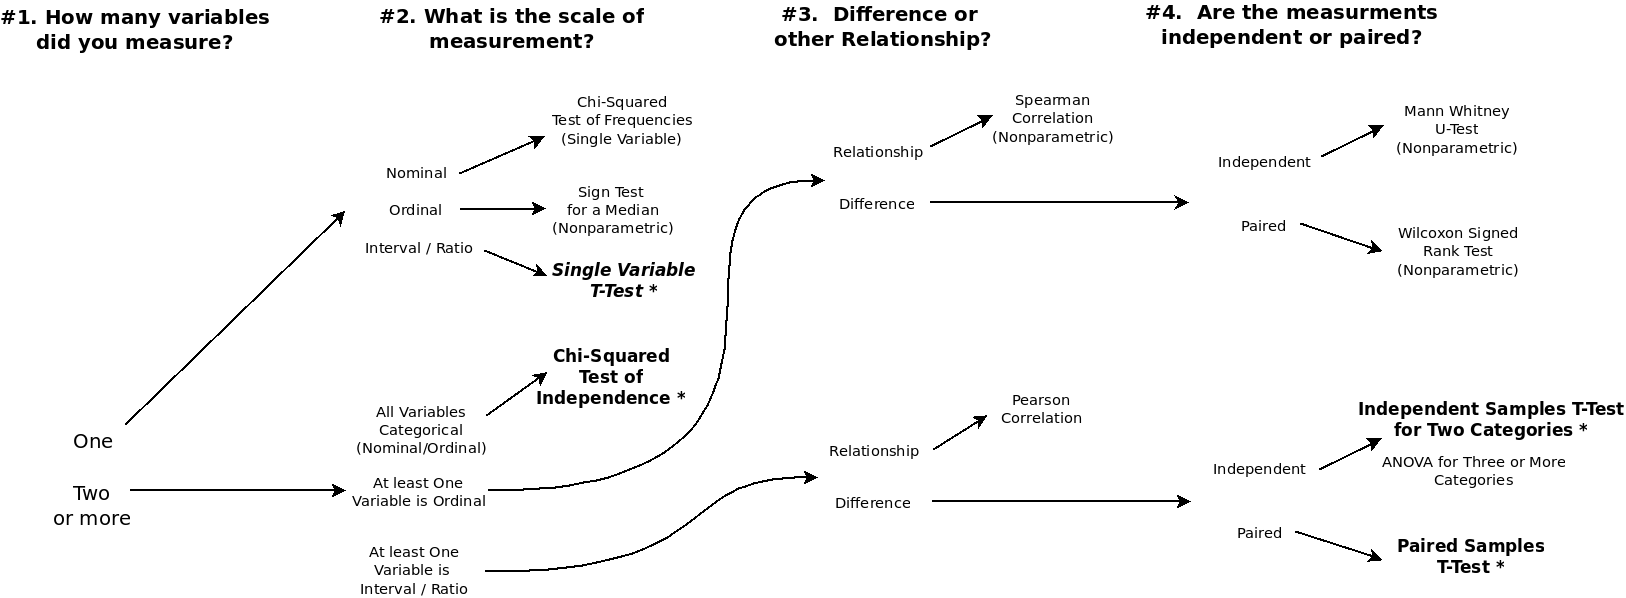
\includegraphics[scale=0.37]{./decisiontree.png}
\end{sidewaysfigure}

After presenting the decision tree, the students were asked to put away their notes so that they could not reference the figure when completing the next two exercises.  The intention of presenting the decision tree is to provide students a mental organization for their existing knowledge of statistical tests, not to provide a physical reference to depend on when tasked with choosing statistical tests.  The students completed the remaining two exercises, and we made the same class observations described above.   We conducted the lesson in three sections of the course, and in each section, we administered the four exercises in a different order.  Every exercise appeared before the decision tree in at least one section and after the decision tree in at least one other section.  This allows us to compare the impact the decision tree has on students' performance and thought processes for each of the exercises.  Of particular interest is whether students' thought processes included the four considerations described in Figure \ref{fg:tree}, whether they did so correctly, and in what order they made these considerations.

To measure how well students retained this knowledge organization, in the following week we gave our students an unannounced quiz and asked them to reconstruct the decision tree from memory.  We evaluated each decision tree and noted whether it included each of the four considerations described in Figure \ref{fg:tree}, and whether or not students arrived at each of the four statistical tests without any incorrect considerations.

\section{Initial Lesson Results}
In this section we describe our lesson study experience in Fall 2011.  In the first subsection we discuss student performance on the four exercises, both before and after our intervention that introduced them to a statistical decision tree.  This subsection focuses on summary statistics and discussion based on evidence from students worksheets.  In the second subsection, we describe our experience and findings from observing our students' discussions.

\subsection{Student Performance}
The first row of Table \ref{tb:results} reports the percentage of students who correctly answered each exercise, before and after the decision tree was presented.  Each exercise is described in Appendix A, and each is identified in the table by the statistical test appropriate for the research question.  The percentage of students correctly identifying each statistical test before and after introducing the decision tree reveal general improvement.  The improvement may be for two reasons.  First, the students may simply improve after practice with each subsequent exercise.  Secondly, the decision tree may have helped students better understand the statistical tests and given them a more effective mental organization from which to draw this knowledge.  We examine this possibility more deeply below when we determine what considerations students used in their decision for each scenario.  

\begin{table}\caption{Results on Students' Performance and Considerations}\label{tb:results} \vspace*{1pc}
\begin{tabular}{p{2.05in}|cc|cc|cc|cc} 
\multicolumn{1}{c}{}  & \multicolumn{2}{p{0.9in}}{} & \multicolumn{2}{p{0.9in}}{\centering Independent} & \multicolumn{2}{p{0.9in}}{\centering Paired} & \multicolumn{2}{p{0.9in}}{} \\
\multicolumn{1}{c}{}  & \multicolumn{2}{|p{0.9in}|}{\centering One-Sample} & \multicolumn{2}{|p{0.9in}|}{\centering Samples} & \multicolumn{2}{|p{0.9in}|}{\centering Samples} & \multicolumn{2}{|p{0.9in}}{\centering Chi-Square} \\ \hline
  & Before	&	After	&	Before	&	After	&	Before	&	After	&	Before	&	After	\\ \hline
Percentage Correct (\%)	&	77	&	82	&	54	&	100	&	0	&	67	&	86	&	58	\\  \hline
Number of Variables (\%)    &	83	&	100	&	91	&	100	&	95	&	97	&	91	&	100	\\ 
Considered Correctly (\%)	&	71	&	82	&	91	&	100	&	82	&	94	&	91	&	100	\\ \hline
Scale of Measurement (\%) 	&	57	&	86	&	83	&	95	&	91	&	83	&	64	&	94	\\ 
Considered Correctly (\%)	&	57	&	73	&	71	&	68	&	91	&	83	&	64	&	72	\\ \hline
Independent/Paired (\%)	&	6	&	27	&	26	&	64	&	18	&	83	&	5	&	19	\\ 
Considered Correctly (\%)	&	94	&	73	&	17	&	59	&	0	&	61	&	95	&	81	\\ \hline
Difference/Comovement (\%)  &	6	&	5	&	49	&	82	&	50	&	22	&	82	&	50	\\
Considered Correctly (\%)	&	94	&	95	&	37	&	73	&	50	&	22	&	73	&	33	\\ \hline
Sample Size*	        &	35	&	22	&	35	&	22	&	22	&	36	&	22	&	36	\\  \hline
\multicolumn{9}{p{6.5in}}{\footnotesize{* Sample size is number of students who completed the exercise. As students discussed the problems in groups, this does not represent a number of independent observations.}} \\
\end{tabular}
\end{table}

The overall percentage correct reveals the paired-samples t-test was the most difficult for students.  Interestingly, none of the 22 students who were given this question before the decision tree intervention answered this question correctly.  Following the intervention, 67\% of students answered it correctly.  

The percentage correct for the Chi-squared test of independence shows that student performance actually decreased after the decision tree intervention.  About 86\% of students answered this question correctly before the intervention, and only 58\% afterward.  The most common incorrect answer for this question was a Pearson correlation coefficient, another test that examines a relationship between two variables, but used for interval/ratio data rather than categorical data.  Classroom observations revealed that this decision was based on the word ``relationship'' appearing in the exercise, and even though many students correctly established that the scale of measurement for the relevant variables were nominal, they still often drew the wrong conclusion.

Table \ref{tb:results} also describes the overall percentage of students that considered each of the following factors in their written responses: 1) the number of variables involved in the research question, 2) the scale of measurement for the given variables, 3) the intent of the statistical test (i.e., whether the method tests for differences or a relationship between two variables), and 4) independent versus paired samples.  The table also reports what percentage of students made the correct determination when considering a factor.  

For the most part, students did consider the number of variables and the scale of measurement of the variables.  Recognizing whether or not samples were independent or paired and whether the scenario suggested examining differences or a relationship occurred less frequently, and had mixed results by test.  We can see that the decision tree did lead to an improvement in this aspect of students' thought processes.  Before introducing the decision tree, less than half of the students (49\%) considered whether a test for a difference or relationship was appropriate, and about one-forth (26\%) considered whether the samples were independent or paired.  Following the decision tree, the percentage of students considering difference versus relationship increased to 82\% and the percentage of students considering independent versus paired samples increased to 64\%.  This is associated with an increase from 54\% of students correctly answering this question before the intervention to 100\% of students correctly answering this question after the intervention.  Regarding the paired-samples t-test, following the intervention, students were more likely to consider independent versus paired samples, but were less likely to consider whether a test involved taking differences or looking for a relationship.

\begin{table}\caption{Level of Confidence for Students Answering Correctly and Incorrectly}\label{tb:confidence}\vspace*{1pc}
\begin{tabular}{p{1.5in}|ccc|ccc} 
\multicolumn{1}{c}{} & \multicolumn{3}{c}{Correct Responses} & \multicolumn{3}{c}{Incorrect Responses} \\[0.5pc]
 & \multicolumn{1}{p{0.71in}}{\vspace*{-2pc}\begin{center}Not Confident (\%)\end{center}\vspace*{-2pc}}
 & \multicolumn{1}{p{0.71in}}{\vspace*{-2.5pc}\begin{center}Somewhat Confident (\%)\end{center}\vspace*{-2pc}}
 & \multicolumn{1}{p{0.71in}}{\vspace*{-2pc}\begin{center}Very Confident (\%)\end{center}\vspace*{-2pc}}
 & \multicolumn{1}{|p{0.71in}}{\vspace*{-2pc}\begin{center}Not Confident (\%)\end{center}\vspace*{-2pc}}
 & \multicolumn{1}{p{0.71in}}{\vspace*{-2.5pc}\begin{center}Somewhat Confident (\%)\end{center}\vspace*{-2pc}}  
 & \multicolumn{1}{p{0.71in}}{\vspace*{-2pc}\begin{center}Very Confident (\%)\end{center}\vspace*{-2pc}}  \\ \hline
One-Sample & 0 & 40 & 60 & 8 & 83 & 8 \\
Independent Samples & 10 & 46 & 44 & 0 & 69 & 31 \\
Paired Samples & 4 & 46 & 50 & 28 & 66 & 6 \\
Chi-Square & 3 & 60 & 38 & 24 & 29 & 47 \\ \hline
\end{tabular}
\end{table}

Table \ref{tb:confidence} describes the level of student confidence by statistical test and whether the student answered each problem correctly or incorrectly.  Students who gave correct responses were generally ``somewhat confident'' or ``very confident'' for each test.  Students who gave incorrect responses were more likely to indicate a lack of confidence for the paired sample t-test and the Chi-square test of independence.  Still, over 30\% of students that incorrectly answered the independent-samples t-test question felt ``very confident'' about their responses, and over 47\% of the students that incorrectly answered the Chi-square test question felt ``very confident.''  This suggests that many students do not recognize the weaknesses in their understanding regarding these research questions.

\begin{table}\caption{Students' Decision Trees}\label{tb:trees}\vspace*{1pc}
\begin{tabular}{l|c||l|c}
Statistical Test & Percent Correct & Trait Considered & Percent Included \\ \hline
One Sample & 72 & Number of Variables & 93 \\
Independent Samples & 67 & Scale of Measurement & 89 \\
Paired Samples & 51 & Independent / Paired & 54 \\
Chi-Square & 65 & Difference / Relationship & 53 \\ \hline
\end{tabular}
\end{table}

Table \ref{tb:trees} describes the students' presentation of the decision tree, drawn from memory one week following our lesson study classroom observation.  It includes the percentage of students that identified each of the four statistical tests without any incorrect information and the percentage of students that included each of the four considerations.  A branch was labeled as correct even if it was missing some considerations leading up to the statistical test, just so long as the considerations that were made were done correctly.   Almost all students included the number of variables and the scale of measurement in their decision trees.  Only half of the students included the two, seemingly more difficult concepts, of independent versus paired samples and whether a test is for a difference or relationship.  Overall, the students did recall the four statistical tests.  However, considering the lack of inclusion of some considerations in the decision tree, as well as the fact that many students did not include all four statistical tests in their tree, it is evident that the complete organizational structure had largely not yet been internalized.  There were a small number of students, though, that were able to correctly reconstruct the entire decision tree from memory.

\subsection{Classroom Observations}

In this section, we describe more about students thought processes as evident from our experience sitting with the students and documenting their conversations.  

Students largely considered scale of measurement, both before and after the decision tree intervention.  Often, they did not mention scale of measurement so explicitly, but instead implied it with a discussion of what could be calculated with the data.  For example, many students observed that the data could be used to calculate a mean, implying the scale was interval or ratio.  Students often had difficulty with the concept of paired versus independent samples.  It is unclear whether students did not consider this factor because they did not understand the difference, or because they did not understand the importance of this distinction in identifying the appropriate statistical test.  

Following the decision tree intervention, many students used a process of elimination to come to a conclusion.  Sometimes students eliminated a test because it had already been used to answer a previous question.  Sometimes students used what appeared to be a quite random process of elimination, where they started with any test they could remember and tried to find reasons to eliminate it.  More substantially though, some students used the process of elimination by considering a factor present in the decision tree and then eliminated tests on the basis of that factor.  For example, sometimes students identified that a problem concerned a ratio variable and thereby eliminated the Chi-square test of independence.  This is a reasonably good strategy, but the discussion indicated that there were factors in the decision tree that they were more comfortable with than others.

We also found that sometimes the decision tree caused more confusion, at least initially.  In some cases students asked the right set of questions, but many times were not able to answer these correctly, and were unable to reach the correct conclusion.  When observing the order of the factors that students considered, it rarely followed the order that the tree presented, even after the decision tree was introduced.  We also found that students often did not pause to reflect on the purpose or intent of the research question first, and sometimes never at all.  

Both before and after the intervention, we identified sources of confusion regarding statistical language.  The first, as we mention above, is the word, ``independent'' to describe samples with different observations in each sample.  Secondly, students had confusion identifying what should be considered a variable.  For example, with the scenario regarding independent-samples, students were asked to determine whether the number of hours students spend studying (ratio variable) is different between students that are employed versus those who are not employed.  Many times, students identified employment status as a nominal variable, which is appropriate.  But when considering an independent-samples t-test, some rejected the idea because that was a test for differences in means, which concerns two ratio variables.  

Finally, students struggled with the colloquial use of the term, ``relationship.''  In the problem for the Chi-Squared tests of independence, students were asked to determine the relationship between employment status (given in three categories) and class standing (given in four categories).  Many students peevishly hung on to the word ``relationship'' and used it as a basis for deciding that a Pearson correlation test was appropriate.  

In the next section, we expand upon the problems caused by statistical and colloquial language used in a statistics class.  We focus specifically on how we can alter our lesson to help students better understand statistical language with precise meanings, and to accept colloquial terms without letting it adversely affect their decisions regarding appropriate statistical tests.

\section{Issues with Statistics Language}

We discovered that the choice of statistical language, and the interaction of statistical and colloquial language, can cause confusion when students ask themselves a standard set of questions that are intended to help select an appropriate statistical test for a research question. 

\subsection{Defining Variables}

A fundamental source of confusion concerns what should be considered a variable, especially when a research question involves comparing a measurement across two or more groups.  In the example where students compared GPA between students who were employed versus students who were not employed, there are two correct ways to define the variables of interest.  The first is a nominal / ratio pair: employment status and GPA; the second is a ratio / ratio pair: GPA for employed students and GPA for not-employed students.  

Both pairings are equivalent, but each construction is convenient in different circumstances.  When the research question involves two independent samples, as in the example above, the nominal / ratio pairing aligns with how SPSS treats the data in its spreadsheet columns.  The nominal / ratio paring is a also convenient mental model for thinking about the degrees of freedom, as it is equal to the sample size of the ratio variable minus the number of categories of the nominal variable.  The ratio / ratio pairing is a convenient mental model when using statistical notation, such as when constructing the null hypothesis, $H_0:~ \mu_1 - \mu_2$, or using measures such as $\bar{x}_1 - \bar{x}_2$ in calculation of the t-statistic.  The ratio / ratio mental model is also convenient for determining whether it is appropriate to use an independent-samples test or a paired-samples test, because students can go back to their understanding of independence and correlation to compare the two ratio variables.    

When analyzing paired-samples, the ratio / ratio pairing is arguably the most convenient model.  Both SPSS and Excel treat the data in this way in its spreadsheet columns, the sample size of either of the ratio variables (they are equal in paired-samples) is related to the degrees of freedom, and the model is again beneficial when using statistical notation.

We find both strategies of defining variables can be useful, and we want to prepare our students to be able to choose the right statistical method regardless of how data might be presented to them after they leave the class.  Of particular importance is that they recognize each possibility, and that beginning with one pairing does not lead them down a wrong path for choosing a statistical test.  For example, in our classroom observation we found that when students identified one variable as a nominal variable, some were reluctant to proceed to either the independent-samples or paired-samples t-tests because these involve taking differences between two ratio variables.

\subsection{Three Uses of ``Independence''}

A second source of confusion concerned the use of the term, ``independence.''  By the end of the semester, students are exposed to at least three seemingly different uses of the word.  Early in the semester when we discuss causal research, we introduce the idea of independent versus dependent variables. We return to this idea later in the course when discussing correlation and regression analysis.  In this case, the word ``independent'' describes a single variable, i.e. the explanatory variable.  An expert would recognize in the regression context that an independent variable and a dependent variable are in fact not jointly independent.  An expert would also recognize that multiple independent variables in a multiple regression analysis can be dependent on one another (we call this multicolinearity).  One can see how this could lead to a confusing conclusion for a statistics novice that an independent variable is not independent.  

The idea of independence comes up again when discussing the Chi-squared test of independence for two categorical variables.  In this case, the word describes the relationship between two variables, and the test itself is used to determine the presence of dependence.  An expert can certainly see the same is true of correlation or regression analysis, but the use of the word, ``independent'' was used to describe a single variable, and that designation remains despite the results of the statistical analysis.

Finally, the term comes up again to describe two different samples, and is used to determine whether one should choose an independent-samples t-test or paired-samples t-test (or between-effects ANOVA and repeated-measures ANOVA for multiple variables).  The types of research questions behind these tests do not involve ideas of co-movement between the variables, and the statistical tests do not determine a presence of dependence like the Chi-squared test of independence.  To the novice, this term appears to be completely different than the previous uses of the word.  The novice might simply memorize that independent samples means different observations are in each sample and the only other option is paired samples, where exactly the same observations are in each sample.  Too often, though, students get distracted by the word, ``independent'' in ``independent samples t-test'' and confuse this idea with the other concepts in the course that use the same word.


\subsection{Colloquial Use of ``Relationship''}

In our classes, we describe the Pearson and Spearman correlation coefficients as measuring a relationship between two variables.  We also used the term ``relationship'' to describe the purpose of the Chi-squared test of independence, though perhaps less so in favor of the word independence.  This becomes problematic because the term relationship can appear colloquially, yet appropriately, for situations in which tests for differences are appropriate.  For example, consider a research question examining the relationship between smoking (measured as smoker or non-smoker) and lung-capacity.  An independent-samples t-test can determine whether there is a difference in mean lung capacity between those that smoke and those that do not.  Such a test does determine a relationship between a nominal variable, smoking status, and a ratio variable, lung capacity, but the appropriate test is one measuring a difference. 

\subsection{Addressing Issues with Statistics Language}
Considering these language issues, we suggest the following carefully worded questions to accompany the statistical decision tree:

\be
\item Always keep in mind, what is your research question.  What did you measure?
\item How many variables did you measure?
\item What is the scale of measurement?  Nominal / Ordinal / Interval / Ratio
\item If you have two or more \textit{measurements}, are you looking for a difference or another relationship?  
  \be
  \item A difference implies comparing two or more measurements, and determining whether they are equal or not.  Keep your research question in mind.
  \item If another relationship, is there co-movement?  That is, is the movement of one variable associated with the movement of another variable?  Keep your research question in mind.
  \ee
\item If you are looking for a difference, are your measurements independent or paired?
  \be
  \item Independence implies that the sample observations, whose two measurements you are differencing, are not related.
  \item If the measurements are not independent, are they paired?  This implies the same observations are used in each measurement.
  \ee
\ee

\section{Revised Lesson Results}
Lesson studies typically involve two or more iterations, taking place over multiple terms.  Subsequent iterations use what instructors learned in the previous iteration to make evidence-based improvements in the lesson and/or in teaching practices (\citeauthor{cerbinbook} \citeyear{cerbinbook}, Chapter 6).  We made three significant changes to our teaching practices in Spring 2012.  First, we were more careful and explicit about colloquial and statistical language.  Secondly, we presented a more careful wording of the decision tree questions as suggested in the previous section.  Finally, and perhaps most substantially, we began the unit on statistics with the development of the decision tree and we referred to the decision tree for several class periods throughout the unit.  \citet{ausubel1978} suggests that student learning is improved when instructors share a way to organize knowledge of upcoming material.  We expect using the decision tree throughout the unit allows students to internalize the organizational structure, and therefore help them be better able to use it to select statistical tests.

We administered the same set of exercises in Spring 2012; students' performance statistics are reported in Table \ref{tb:spring_results}.  As we used the decision tree throughout the unit, we are not able to make before and after comparisons as we did with Fall 2011.  The results are somewhat disconcerting.  Comparing the first row of summary statistics to the first row in Table \ref{tb:results}, we see that in Spring 2012, students performed only about as well as the the previous semester's students who had not yet been introduced to the decision tree.   Concerning the Chi-Square test, in Spring 2012 students performed worse on average than in Fall 2011.

The remaining rows in Table \ref{tb:spring_results} describe the overall percentage of students that considered each of the four factors in the decision tree in their written responses.  In most cases, the students in Spring 2012 semester were more likely to consider each factor in their decision compared to the students in Fall 2011, and they were more likely consider it correctly.  Still, as is evident from the first row in the table, this did not always translate into a higher percentage of correct answers. 

\begin{table}\caption{Revised Lesson: Results on Students' Performance and Considerations}\label{tb:spring_results} \vspace*{1pc}
\begin{tabular}{p{2.05in}|c|c|c|c}
\multicolumn{1}{c}{}  & \multicolumn{1}{p{0.9in}}{} & \multicolumn{1}{p{0.9in}}{\centering Independent} & \multicolumn{1}{p{0.9in}}{\centering Paired} & \multicolumn{1}{p{0.9in}}{} \\
\multicolumn{1}{c}{}  & \multicolumn{1}{|p{0.9in}|}{\centering One-Sample} & \multicolumn{1}{|p{0.9in}|}{\centering Samples} & \multicolumn{1}{|p{0.9in}|}{\centering Samples} & \multicolumn{1}{|p{0.9in}}{\centering Chi-Square} \\ \hline
Percentage Correct (\%)	&	92 & 56 & 47 & 29 \\  \hline
Number of Variables (\%)    & 96 & 96 & 100 & 95		\\ 
Considered Correctly (\%)   & 90 & 95 & 100 & 95	\\ \hline
Scale of Measurement (\%)  	& 71 & 96 & 92 & 86		\\ 
Considered Correctly (\%)	& 69 & 83 & 86 & 32		\\ \hline
Independent/Paired (\%)	&	4 & 49 & 84 & 2		\\ 
Considered Correctly (\%)	& 96 & 42 & 55 & 98		\\ \hline
Difference/Comovement (\%)  & 0	& 60 & 80 & 77		\\
Considered Correctly (\%)	& 100 & 50 & 80 & 69 		\\ \hline
Sample Size	        &	84 & 84 & 84 & 84	\\  \hline
\end{tabular}
\end{table}

Again in Spring 2012 we had our students recreate the decision tree from memory.  The students performance on this exercise is reported in Table \ref{tb:spring_trees}.  Comparing these results with Table \ref{tb:trees}, we find that retention of the decision tree was much better in Spring 2012 than the previous semester.  Most students included all four tests with no wrong information in the branches leading to the test, and a large majority of students remembered all four factors to consider when choosing a statistical test.  While not reported in the table, we also found that a large number students were able to recreate the entire decision tree without any errors, which included many more tests than the four examined in this lesson.

\begin{table}\caption{Revised Lesson: Students' Decision Trees}\label{tb:spring_trees}\vspace*{1pc}
\begin{tabular}{l|c||l|c}
Statistical Test & Percent Correct & Trait Considered & Percent Included \\ \hline
One Sample & 89 & Number of Variables & 99 \\
Independent Samples & 76 & Scale of Measurement & 100 \\
Paired Samples & 73 & Independent / Paired & 84 \\
Chi-Square & 83 & Difference / Relationship & 89 \\ \hline
\end{tabular}
\end{table}

Overall when comparing performance in Spring 2012 to Fall 2011, we find that students did have better retention of the decision tree and were more likely to use the decision tree questions to choose a statistical test.  Unfortunately, we failed to find evidence that this translated to better performance picking an appropriate statistical test to answer a research question.  Average student performance typically does vary from one semester to the next, from one section to the next, and from one instructor to the next, so it is difficult to attribute specific reasons for declines or improvements in student performance comparing over semesters.  Still, we expect we do have a valuable teaching tool to help students understand the inter-relationships between statistical tests, which can help students' long-run retention.  For the students in three of the four sections, this lesson was one of the first instances that the students were expected to choose an appropriate statistical test, given a scenario.  Previous lessons focused on individual statistical tests and how to conduct the analyses in SPSS.  We expect sustained practice using the decision tree to choose statistical tests will lead to further improvements in student learning in this area.

\section{Conclusions} 
One of the most valuable insights that we gained from this lesson study was the teaching strategy we employed in Spring 2012 that led to significant retention of the statistical decision tree.  We used this knowledge organization throughout the unit on statistics which allowed students to see how statistical methods were connected to each other, and under what circumstances it is appropriate to each test.  Unfortunately, we failed to find evidence in Spring 2012 that this led to an immediate improvement in student performance on the in-class exercises.  Still we found students had a strong retention of the mental mapping, which with continued practice is likely to lead to an improvement in long-run performance applying statistical methods.  Students that have retained a way to organize knowledge of statistics will also likely have an enhanced ability to learn and retain new statistical methods that they may come across in the future.  The knowledge organization gives them an ability to connect new ideas to an existing body of knowledge.

Our lesson also made the students' learning and thinking process visible, which revealed some unexpected sources of confusion among students.  We discovered some students had problems on how to define variables, which led to errors in picking an appropriate statistical test.  We also found the interaction between colloquial and statistical language created confusion for many students.  We analyze these problems in some detail in this paper and make suggestions for addressing them in the classroom.

\newpage

\app\appsection{In-class Exercises}

\noindent \textbf{Directions:} You will be given four research questions involving the survey questions below.  Work in your groups to answer the questions when prompted.  All papers will be collected. \\

\noindent \textbf{Scenario:} A researcher is interested in exploring the relationship between student unemployment and effort put forth towards academics.  She administers a survey to full-time University of Wisconsin - La Crosse (UW-L) undergraduate students which includes the following questions:
\be
\item What is your employment status?
\bi \item Full time \item Part time \item Not Employed \ei
\item On average, how many hours do you work per week? (Numeric / open ended)
\item On average, how many hours to you study per week? (Numeric / open ended)
\item What is your class standing? \bi \item Freshman \item Sophomore \item Junior \item Senior \ei
\ee

\noindent \textbf{Exercise A} \\
Suppose the national average for the number of hours full-time college students work is 12 hours per week.  The researcher is interested in determining if there is evidence that UW-L students work on average more hours than the national average?
\be
\item What statistical method / test would you use to answer this question?
\item Explain your reasoning for the previous answer.  What characteristics of this research question and methodology make the test you chose appropriate?
\item How confident are you that your answer to the previous two questions is correct?  
\bi \item Very Confident \item Somewhat Confident \item Not Confident \ei
\ee

\noindent \textbf{Exercise B}\\
The researcher is interested in determining whether there is a difference in the average number of hours students study per week between those who are employed (either full-time or part-time) and those who are not employed.
\be
\item What statistical method / test would you use to answer this question?
\item Explain your reasoning for the previous answer.  What characteristics of this research question and methodology make the test you chose appropriate?
\item How confident are you that your answer to the previous two questions is correct?  
\bi \item Very Confident \item Somewhat Confident \item Not Confident \ei
\ee

\noindent \textbf{Exercise C} \\
The researcher is interested in determining whether there is a relationship between class standing and employment status.
\be
\item What statistical method / test would you use to answer this question?
\item Explain your reasoning for the previous answer.  What characteristics of this research question and methodology make the test you chose appropriate?
\item How confident are you that your answer to the previous two questions is correct?  
\bi \item Very Confident \item Somewhat Confident \item Not Confident \ei
\ee

\noindent \textbf{Exercise D}\\
The researcher is interested in determining whether on average students spend more hours studying than the number of hours students spend working.
\be
\item What statistical method / test would you use to answer this question?
\item Explain your reasoning for the previous answer.  What characteristics of this research question and methodology make the test you chose appropriate?
\item How confident are you that your answer to the previous two questions is correct?  
\bi \item Very Confident \item Somewhat Confident \item Not Confident \ei
\ee

\newpage
\appsection{Classroom Observation Guide}
Observe the group discussion about the statistical test which is appropriate to answer the question. Record each observation with a number to indicate the order that the students consider each element. They may circle around to an element more than once, record this as it happens (i.e. any element may have more than one number beside it). If the conclusion about the element is incorrect, record an X by the number. 

\noindent \textbf{Exercise (circle) A B C D} \\
\noindent \textbf{Observation number (circle) 1 2 3 4} \\

\begin{tabular}{|p{4.5in}|l|} \hline
Element & Consideration \\ \hline
Discuss the number of variables considered. & \\ \hline
Discuss the scale of measurement. & \\ \hline
Discuss whether variables are independent or not. & \\ \hline
Reflect on the purpose or intent of statistical test (for example they talk about determining the difference or relationship). & \\ \hline
Other & \\ \hline
\end{tabular} \\

\noindent Other questions to consider: 
\be
\item Did the students take into account any irrelevant considerations?
\item Did the students reach the correct conclusion without well articulated reasons?
\item Did students reach the incorrect conclusion, yet used mostly correct and well articulated reasons?
\item How many group members were actively engaged in the conversation? (Include those who are actively listening to understand the concepts, but not those just trying to write the correct answer).
\ee

\newpage
\nocite{*}
\begin{singlespace}
\bibliographystyle{apecon}
\bibliography{bus230ls}
\end{singlespace}



\end{document}



